\documentclass[border=3mm]{standalone}
\usepackage{pgfplots}
\pgfplotsset{compat=newest}
\pagestyle{empty}
\begin{document}
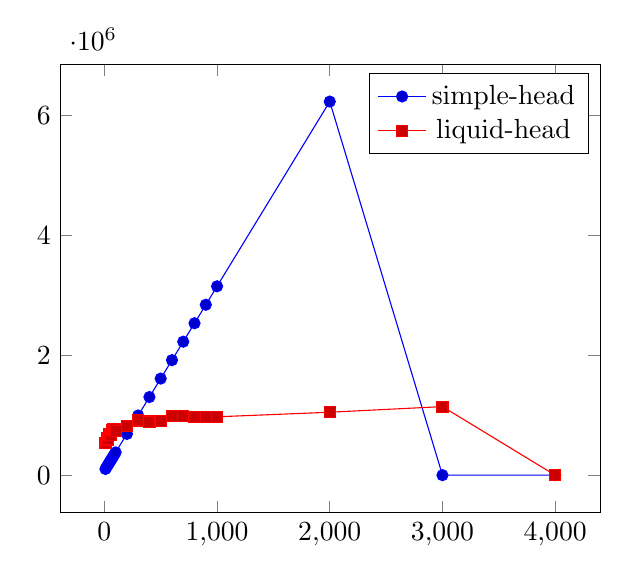
\begin{tikzpicture}
\begin{axis} 
\addplot  plot coordinates {
(10, 103692)
(20, 134473)
(30, 165254)
(40, 196036)
(50, 226818)
(60, 257601)
(70, 288384)
(80, 319167)
(90, 349951)
(100, 380735)
(200, 688599)
(300, 996502)
(400, 1304444)
(500, 1612425)
(600, 1920444)
(700, 2228503)
(800, 2536601)
(900, 2844739)
(1000, 3152915)
(2000, 6236825)
(3000, 0)
(4000, 0)
};\addplot  plot coordinates {
(10, 536968)
(20, 613237)
(30, 595379)
(40, 689505)
(50, 666551)
(60, 671584)
(70, 760741)
(80, 765774)
(90, 763257)
(100, 742819)
(200, 819088)
(300, 913534)
(400, 895548)
(500, 898193)
(600, 989610)
(700, 992255)
(800, 971817)
(900, 966912)
(1000, 974398)
(2000, 1050794)
(3000, 1144856)
(4000, 0)
};\legend{simple-head,liquid-head}
\end{axis}
\end{tikzpicture}
\end{document}